
% --------------------------------------------------------------
% This is all preamble stuff that you don't have to worry about.
% Head down to where it says "Start here"
% --------------------------------------------------------------

\documentclass[11pt]{article}

\usepackage{bera}
%\renewcommand{\familydefault}{\rmfamily}

\usepackage{graphicx,url}
\usepackage{proof}
\usepackage{framed}
\usepackage{etaremune}
\usepackage{hyperref}
\usepackage{url}
\usepackage[margin=1in]{geometry}
\usepackage{amsmath,amsthm,amssymb,amsfonts}
\usepackage{paralist}
\thispagestyle{empty}
\hypersetup{
    colorlinks=true,
    linkcolor=blue,
    filecolor=magenta,      
    urlcolor=blue,
    pdftitle={Overleaf Example},
    pdfpagemode=FullScreen,
    }

% 1. To get version suitable for students to populate,
%    remove the contents of the \ignoreSoln{..body..}
%
% 2. To get a version suitable for generating PDF 
%    without solutions, remove the #1 below
%
% 3. To generate solutions, keep the #1 below
%
% 4. Assigned grader fills \ignoreSoln{..body..}
%    and also provides his/her feedback to student
%    and policy followed for point deduction
%    So design policy before grading begins.

\newcommand{\ignoreSoln}[1]{#1}   
%\newcommand{\ignoreModel}[1]{#1} 


\newcommand{\bigset}[2]{\big\{\;#1\;:\;#2\;\big\}}
\newcommand{\N}{\mathbb{N}}
\newcommand{\Z}{\mathbb{Z}}
\newcommand{\R}{\mathbb{R}}
\newcommand{\Np}{\mathbb{N^{+}}}

\newenvironment{theorem}[2][Theorem]{\begin{trivlist}
\item[\hskip \labelsep {\bfseries #1}\hskip \labelsep {\bfseries #2.}]}{\end{trivlist}}
\newenvironment{lemma}[2][Lemma]{\begin{trivlist}
\item[\hskip \labelsep {\bfseries #1}\hskip \labelsep {\bfseries #2.}]}{\end{trivlist}}
\newenvironment{exercise}[2][Exercise]{\begin{trivlist}
\item[\hskip \labelsep {\bfseries #1}\hskip \labelsep {\bfseries #2.}]}{\end{trivlist}}
\newenvironment{reflection}[2][Reflection]{\begin{trivlist}
\item[\hskip \labelsep {\bfseries #1}\hskip \labelsep {\bfseries #2.}]}{\end{trivlist}}
\newenvironment{proposition}[2][Proposition]{\begin{trivlist}
\item[\hskip \labelsep {\bfseries #1}\hskip \labelsep {\bfseries #2.}]}{\end{trivlist}}
\newenvironment{corollary}[2][Corollary]{\begin{trivlist}
\item[\hskip \labelsep {\bfseries #1}\hskip \labelsep {\bfseries #2.}]}{\end{trivlist}}

\DeclareMathSizes{14}{14}{14}{14}

\begin{document}

% --------------------------------------------------------------
%                         Start here
% --------------------------------------------------------------

%\renewcommand{\qedsymbol}{\filledbox}
\newlength{\minpagw}
\settowidth{\minpagw}{\hspace{40em}}

\begin{center}
\begin{large}
  CS 6110, Spring 2022, Assignment 4  \\
  Given 2/11/22 -- Due 2/18/22 by 11:59 pm via your Github 
  \ \\
%  \ \\  
    {  {\Large\bf NAME: Tripti Agarwal } \hfill {\Large\bf UNID: u1319433}\hspace{4cm} }
          \ \\
\end{large}

\end{center}


\begin{enumerate}
  
%- 1 ----------------------------------------------------------------
\item \textbf{(50 points - 25 for pre and 25 for partial - Alloy)}
\begin{figure}
\begin{minipage}{\minpagw}
  \fbox{%
    \parbox{\linewidth}{%
     \begin{enumerate}
         \item sig S is a signature where pre is a binary relation over S.
         \item Different models are generated at this point which have one or more relations with S.
         \item \textbf{Preorder facts and output} Pre order is the order such that it is reflexive and transitive.\\
         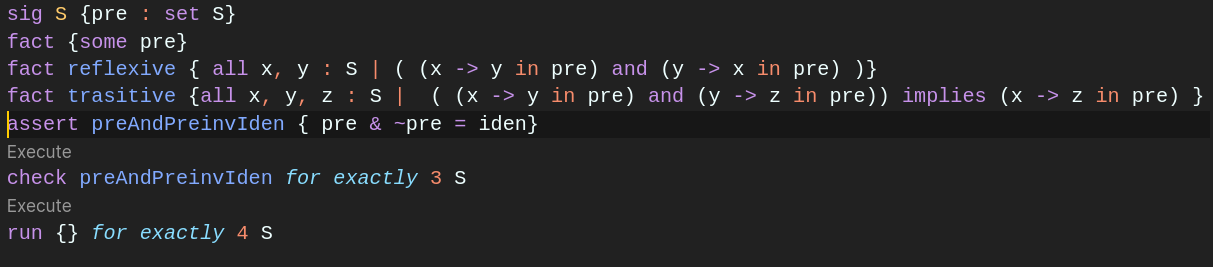
\includegraphics[width=7.0in]{Q1_pre.png}\item The check did not pass as iden has more relation than pre and ~pre.\\
         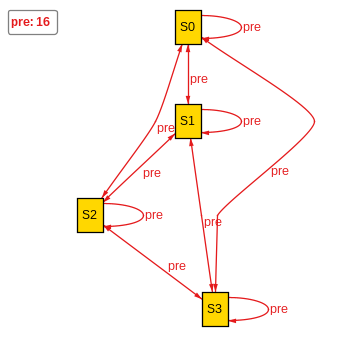
\includegraphics[width=3.0in]{Q1_pre_output.png}
         
         \item \textbf{Partial order facts and output} Partial order is a preorder with anti-symmetry\\
         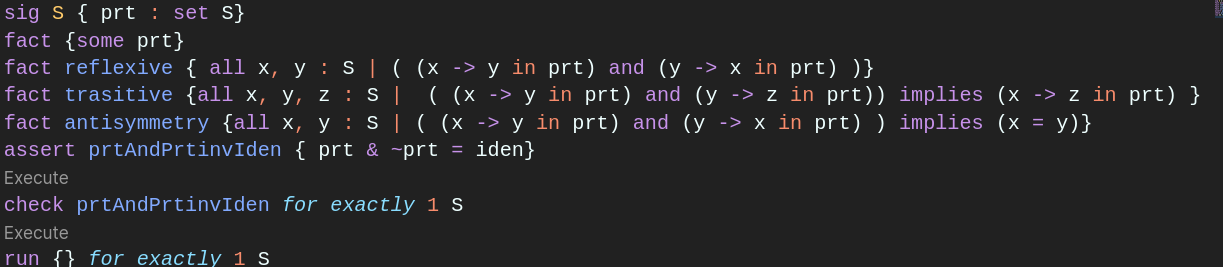
\includegraphics[width=7.0in]{Q1_part.png}
         \item The check did not pass as iden has more relation than part and ~part.\\
         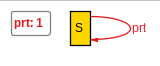
\includegraphics[width=3.0in]{Q1_part_output.png}
     \end{enumerate}
    }%
  }%
  \end{minipage}
\end{figure}
\newpage
%- 2 ----------------------------------------------------------------
\item 
  \textbf{Peterson TSO}
\begin{figure}
\begin{minipage}{\minpagw}
  \fbox{%
    \parbox{\linewidth}{%
      \begin{itemize}
          \item Memory ordering describes the order of accesses to computer memory by a CPU. Most programming languages have some notion of a thread of execution which executes statements in a defined order.
         \item Processors	use	write	buffers	to	hold	committed	stores	until	the	memory	system	can	 process	them. A	store	enters	the	write	buffer	when	the	store	commits,	and	a	store	exits	the	write	
buffer	when	the	block	to	be	written	is	in	the	cache	in	a	read–write	coherence	state.		
\item For	a	single-core	processor a	write	buffer	can	be	made	invisible	by	ensuring	that	a	load	returns	the	value	of	the	most	recent	
store	even	if	one	or	more	stores	to	are	in	the	write	buffer. When	building	a	multicore	processor,	it	seems	natural	to	use	multiple	
cores,	each	with	its	own	bypassing	write	buffer.
\item \textbf{TSO} In-order memory operations: Read-to-Read, Read-to-Write, Write-to-Write. Out-of-order memory operations: Write-to-Read (later reads can bypass earlier writes)
\begin{itemize}
    \item Forwarding of pending writes in the store buffer to
successive reads to the same location.  Writes become visible to writing processor first
\item Store buffer is FIFO. Breaks Peterson's algorithm for mutual exclusion
\end{itemize}
\item \textbf{Peterson TSO error} We see that the given code has an error. 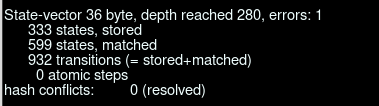
\includegraphics[width=3.0in]{peterson_tso_error.png}
\item The error trace shows that the ncrit value is 2 where as we asserted the value of ncrit as 1. Hence the mutual exclusion of peterson's algorithm is violated.
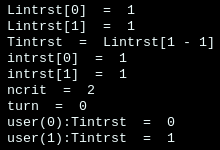
\includegraphics[width=2.5in]{peterson_tso_error_trace.png}
   \end{itemize}
   
    }%
  }%
\end{minipage}
\end{figure} 
\newpage
%- 3 ----------------------------------------------------------------
\item (10 points, The Java example with volatiles)
  Read-up on Java volatiles. Run the example \verb|VBad.java|.
  Insert volatiles selectively (just for req or just for ack).
  Does that correct the apparent hang? (I don't know the answer
  but thought you'd like to try.) To get the apparent hang,
  first you must leave out the volatile totally and get the
  hangs on your machine.
  Then {\em explain the reason for this hang.} (Why might it be
  happening? What reordering in the protocol can cause it to
  change. Assume only store/load reorderings.\footnotemark)
  %
  {\em Then} try to add one volatile
  and see if you get a hang. Explain your observations. (Bound
  your empirical testing to say an hour.)
  %
  \footnotetext{All attempts to read the generated code failed.
    We assume there is no advantage gained by the compiler
    reordering such a short program's instructions. Thus it
    must be the hardware store-buffer and/or cache of the processor.}

  \begin{minipage}{\minpagw}
  \fbox{%
    \parbox{\linewidth}{%
    \begin{itemize}
        \item  We get the hang when ack is not set to volatile.
        \item Volatile in java are like synchronized, atomic wrapper of making class thread-safe. Thread-safe means that a method or class instance can be used by multiple threads at the same time without any problem.
        \item  If both ack and request are not set to volatile, then the value of req and ack keeps changing from true and false and both tid 0 and 1 gets stuck at first and second while loop, respectively.
        \item This means that the request is never getting acknowledged. The code is available on github \href{https://github.com/tripti-agarwal/Formal-Method-verification/blob/main/Assignment4/VBad.java}{link}
    \end{itemize}
      
    }%
  }%
  \end{minipage}
\newpage

%- 4 ----------------------------------------------------------------
\item (10 points, the Man-Wolf-Goat-Cabbage or mwgc game)
\begin{figure}
  \begin{minipage}{\minpagw}
  \fbox{%
    \parbox{\linewidth}{%
      \begin{itemize}
          \item The psuedo code for BFS is available in the following \href{https://github.com/tripti-agarwal/Formal-Method-verification/blob/main/Assignment4/assignment4_Q4.pdf}{pdf}
          \item Yes, the model checker does not infinitely loop and terminate when there is no next state. This is because the terminate variable becomes true and the loop breaks at that point. This is clear from figure 3 and 4 in the  \href{https://www.cs.utah.edu/~kirby/Publications/Kirby-33.pdf}{paper}
          \item We recreate the mwgc example. The example in the class results in an error(code available \href{https://github.com/tripti-agarwal/Formal-Method-verification/blob/main/Assignment4/rivercrossing.m}{here}). The error trace is available here \href{https://github.com/tripti-agarwal/Formal-Method-verification/blob/main/Assignment4/Error_trace_Q4_Given}{error trace}.
          \item 
          The new example have some extra safe state producing no errors (code available \href{https://github.com/tripti-agarwal/Formal-Method-verification/blob/main/Assignment4/rivercrossing_test.m}{here}), as shown in the figure below:\\
          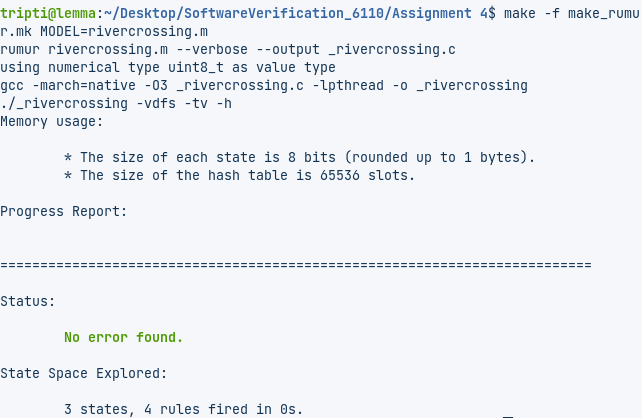
\includegraphics[width=3.0in]{Q4_test.png}\\
          \item The BDD example is satisfiable but not equivalent (code available \href{https://github.com/tripti-agarwal/Formal-Method-verification/blob/main/Assignment4/BDD.ipynb}{here}), as shown below:\\
          \textbf{With given $\rightarrow$ test}
          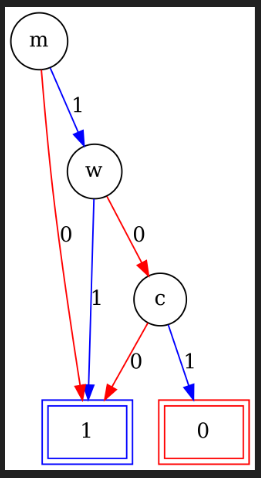
\includegraphics[width=1.0in]{test-given.png}\\
          \textbf{With test $\rightarrow$ Given }
          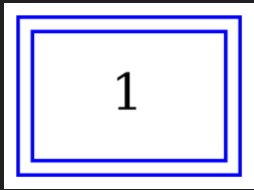
\includegraphics[width=0.5in]{given-test.png}
          
          \item Let say we add another noun 'lion' and change the safe state to "lion can eat wolf" and try to solve the problem, we end up getting a deadlock. This is because none of them can cross the river, without at least one of them eating the other away. Hence this leads to a deadlock. The code is available \href{https://github.com/tripti-agarwal/Formal-Method-verification/blob/main/Assignment4/rivercrossing_safeState_changed.m}{here} and the error trace is available \href{https://github.com/tripti-agarwal/Formal-Method-verification/blob/main/Assignment4/Error_trace_Safestate_changed}{here}.
         
          
      \end{itemize}
    }%
  }%
\end{minipage}  
\end{figure}
 \newpage 
%- 5 ----------------------------------------------------------------  
\item (20 points, DCL)
 \textbf{The "Double-Checked Locking is Broken" Declaration}\\
\begin{minipage}{\minpagw}
  \fbox{%
    \parbox{\linewidth}{%
      \begin{itemize}
          \item C++ codes are dependent on  memory model of the processor, the re-orderings performed by the compiler and the interaction between the compiler and the synchronization library. None of these are specified in C++. In java explicit memory barriers can be used.
          \item \textbf{Non synchoronized code} In multithreaded context, there can be multiple objects that can be allocated and hence we need to synchronize the method.
          \item The above doesn't work, because write can done or percieved out of order. Even if the compiler does not reorder those writes, the memory system reorder those writes and hence can run the thread running in another processor.
          \item Another fix is synchronizing inside an inner synchronized block. The rules of synchronization works that anything inside the synchronized block will work once the lock is released but anything outside can still work, and hence this idea also fails.
          \item Using full bidirectional memory barrier. This idea is inefficient and will not work in java. Also the thread which sees a non-null value for the method field also needs to perform memory barriers. This is because  processors have their own locally cached copies of memory.
          \item \textbf{Making it work for static singleton}
          This guarantees that the field will not be intialized until the field is referenced and that any thread which accesses the field will see all of the writes resulting from initializing that field. This works with 32-bit primitive values but not with 64-bits.
           This is because unsynchronized reads/writes of 64-bit primitives are not guaranteed to be atomic.
           \item \textbf{Using thread local storage}. In this each thread keeps a local flag to determine to determine whether that thread has done the required synchronization. The performanceis dependent on JDK implementation used.
          \item \textbf{Using volatile} In JDK5 we can use volatile, which ensures that the system will not allow write of a volatile to be reordered wrt any previous read or write and a read of a volatile cannot be reordered with respect to any following read or write. 
          \item \textbf{Immutatble objects} Will work without using volatile as well.
      \end{itemize}
    }%
  }%
\end{minipage}    
%- end ----------------------------------------------------------------  


\end{enumerate}

\end{document}
